\documentclass{beamer}[10pt, usepdftitle=false, handout]

\beamertemplatenavigationsymbolsempty

\usepackage[T1]{fontenc}
\usepackage[]{algorithm2e}
\usepackage{multimedia}
\usepackage{gensymb}
\usepackage{textcomp}
%\usepackage{background}
%\backgroundsetup{
%    placement=center,
%    scale=1,
%    contents={The author of this course is PAUL BLONDEL},
%    opacity=0.7
%}
%\setbeamertemplate{background}{\BgMaterial}
%\usepackage[font=small,labelfont=bf]{caption} 

\usetheme{Boadilla}

\title{Data Structure 1}
\author[]{Paul Blondel}
\institute[]{CNAM}
\date[]{September 1st, 2018}

\usepackage[style=british]{csquotes}


\def\signed #1{{\leavevmode\unskip\nobreak\hfil\penalty50\hskip1em
  \hbox{}\nobreak\hfill #1%
  \parfillskip=0pt \finalhyphendemerits=0 \endgraf}}

\newsavebox\mybox
\newenvironment{aquote}[1]
  {\savebox\mybox{#1}\begin{quote}\openautoquote\hspace*{-.7ex}}
  {\unskip\closeautoquote\vspace*{1mm}\signed{\usebox\mybox}\end{quote}}


%\setbeamertemplate{headline}
%{
%  \leavevmode%
%  \hbox{%
%  \begin{beamercolorbox}[wd=1.0\paperwidth,ht=2.25ex,dp=1ex,center]{author in head/foot}%
%    \textcolor{green}{- This course has been made by Paul Blondel -} \usebeamerfont{author in head/foot}\insertsubsection
%  \end{beamercolorbox}}%
%  \vskip0pt%
%}


\setbeamertemplate{footline}
{
  \leavevmode%
  \hbox{%
  \begin{beamercolorbox}[wd=.5\paperwidth,ht=2.25ex,dp=1ex,center]{author in head/foot}%
    \usebeamerfont{author in head/foot}\insertsection
  \end{beamercolorbox}%
  \begin{beamercolorbox}[wd=.5\paperwidth,ht=2.25ex,dp=1ex,center]{title in head/foot}%
    \usebeamerfont{title in head/foot} \inserttitle \hspace*{2em}  \insertframenumber{} / \inserttotalframenumber\hspace*{2ex} 
  \end{beamercolorbox}}%
  \vskip0pt%
}

\AtBeginSection[]
{
   \begin{frame}
    \tableofcontents[ 
    currentsection] 
   \end{frame}
}

\begin{document}
	{
	\setbeamertemplate{footline}{
  	\leavevmode%
  	\hbox{%
  	\begin{beamercolorbox}[wd=.5\paperwidth,ht=2.25ex,dp=1ex,center]{author in head/foot}%
  	\end{beamercolorbox}%
  	\begin{beamercolorbox}[wd=.5\paperwidth,ht=2.25ex,dp=1ex,center]{title in head/foot}%
  	\end{beamercolorbox}}%
  	\vskip0pt%	
	} 
	\begin{frame}
	\titlepage
	\end{frame}

	\begin{frame}
	
	\begin{aquote}{Linus Torvalds}
	I will, in fact, claim that the difference between a bad programmer and a good one is whether he 
	considers his code or his data structures more important. Bad programmers worry about the code. Good programmers worry about data structures and their relationships.	
	\end{aquote}	
	
	\end{frame}


	\begin{frame}
		\tableofcontents
	\end{frame}
	}

	\addtocounter{framenumber}{-3}

	\section{Data}	
	\subsection{Data, types and properties}	

    \begin{frame}[label=(first)]
	
	\begin{block}{What is data?}
	Data is the result of a measurement
	\end{block}	
			
	Examples: The diameter of the sun is \textbf{1.39 million kilometers}, the temperature of the room is \textbf{30\degree C}, and so on.
	
	\hfill\break
			
	A data ...
			
	\begin{itemize}
	\item {... is \textbf{simple} or \textbf{complex} (composed of simple data)}	
	\item {... has a \textbf{type} (integer, character, and so on)}
	\item {... has a set of authorized \textbf{instructions}}
	\end{itemize}
	
	Examples: 'hello' is a complex data (composed of simple character data), 30\degree C is a simple integer data. 'hello' * 30 is not authorized, but 2 * 30 is.
		 
			
    \end{frame}

	%\section{Data}	
	\subsection{Units}	

    \begin{frame}
    
	The most common units are: 
	\begin{itemize}
		\item{1 bit (0 or 1)}
		\item{1 byte (or octet) = 8 bits}
		\item{1 KB (or KO) = 1000 bytes\footnote{1 KB is sometimes defined as equal to 1024 bytes, but this definition is no longer valid. In 1998, the International Electrotechnical Commission stated that 1 KB = 1000 bytes and that 1024 bytes = 1 KiB (kibibyte).}}
		\item{1 MB (or MO) = $10^6$ bytes = 1000 KB}
		\item{1 GB (or GO) = $10^9$ bytes = $10^6$ KB = 1000 MB}
		\item{1 TB (or TO) = $10^{12}$ bytes}
	\end{itemize}	 
    
   	Exemple: 'hello' is stored on 5 bytes (each character is stored on 1 byte).
            
	\end{frame}    
    
   	    
	\section{Memory}
	\subsection{Different memories for different usage}
	
	\begin{frame}

	Two main types\footnote{The CPU cache is another interesting memory, it stores copies of data frequently fetched from the main memory. Interesting fact: Graphics Processing Units dedicated to computing can have up to 5 different data storage types.} of data storage:
	\begin{itemize}
	\item {The main memory (Random-access memory or RAM)
		\begin{itemize}
			\item {Storing running softwares and opened documents}	
		\end{itemize}			
	}
	\item {The mass storage memory 
		\begin{itemize}
			\item {Storing installed softwares and all documents}
			\item {Two main technologies on the market: 
				\begin{itemize}
					\item {Hard-disk drive (HDD) (invented in 1954)}
					\item {Solid-state drive (SSD) (invented in 1978)}
				\end{itemize}
			}
		\end{itemize}			
	}
	\end{itemize}
	
	\begin{center}
	\begin{tabular}{c | c | c }
		 & RAM & HDD / SSD \\ \hline
		Access speed & Fast (2000-26600MO/s) & Slow (50-500MO/s) \\
		Storage capacity & Low (4-32GB) & High (256GB - 1TB) \\
		Storage property & Volatile & Not Volatile 
	\end{tabular}
	\end{center}

	\end{frame}

	\subsection{How it works?}

	\begin{frame}    
    
   	\begin{itemize}
   	
	\item {RAM  
		\begin{itemize}
			\item {All the data is stored in an array of memory cells}
			\item {1 bit = 1 memory cell (DRAM: bit stored in a capacitor)}
		\end{itemize}
		\begin{figure}[t]
		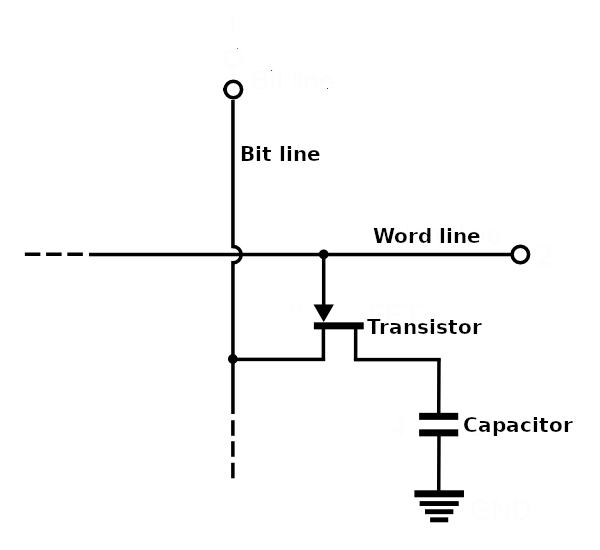
\includegraphics[scale=0.5]{images/ddr_cell.png}
		\vspace*{-0.9em}
		\caption{DRAM memory cell}
		\centering
		\end{figure}
		}
	\item {HDD
		\begin{itemize}
			\item {All the data is stored in disks of ferromagnetic material}
			\item {1 bit = direction of magnetic field lines}			
		\end{itemize}			
				
		\begin{figure}
		\begin{tabular}{cc}
		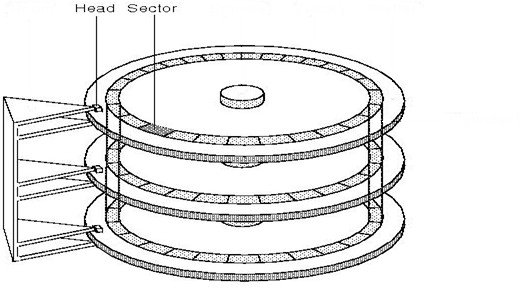
\includegraphics[scale=0.9]{images/hdd_disks.png} &	
		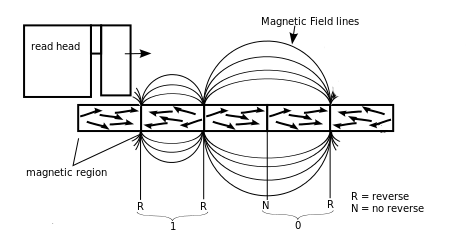
\includegraphics[scale=0.9]{images/hdd_magnetic.png} \\
		\end{tabular}
		\vspace*{-0.5em}
		\caption{Left: disks of ferromagnetic material right: magnetic field lines}
		\end{figure}		
	}
						
	
	\end{itemize}
	
	% the bit of memory is stored in the capacitor, but the capacitor leaks, so it has to be refreshed  each time, that why we call it dynamic 	
	% current in the transistor: the bit line receive the value of the capacitor
	% current in the bit line with 1: we write 1, with 0, we write 0	
	
		   
    \end{frame}
    
	
	\begin{frame}
	
	\begin{itemize}
		\item {SSD 
			\begin{itemize}
				\item{All the data is stored in an array of floating-gate transistors}
				\item{No mechanical moving component = faster}
						
			
			\end{itemize} 
			
	\begin{figure}
		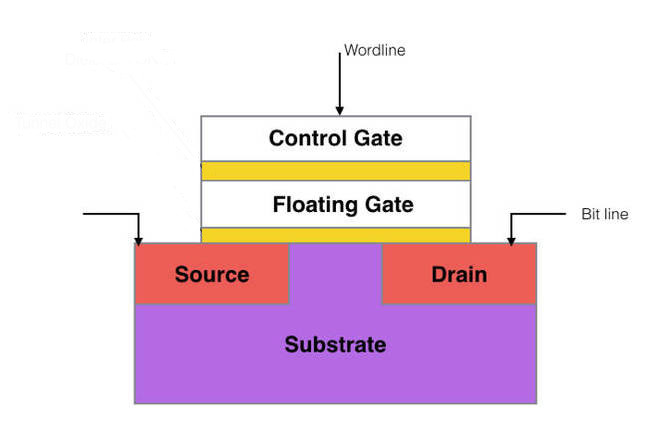
\includegraphics[scale=0.2]{images/floating_gate_flash_cell.jpg} 
     	\vspace*{-0.5em}
		\caption{Floating gate transistor cell}
		\end{figure}			
			
	% The bit is stored in the floating gate, when there is not current in the bit line the bit is tored in the floating gate
			
			}
	
	\end{itemize}
	
	
	\end{frame}    
    

	\section{Algorithm}
	\subsection{What is an algorithm?}

	\begin{frame}
		
	\begin{block}{What is an algorithm?}
	An algorithm is a \textbf{finite sequence of instructions} designed to \textbf{solve a specific problem}. An algorithm is like a cooking recipe. 
	\end{block}	
	
	Writing an algorithm is a preliminary step before coding:
	
	\begin{itemize}
		\item {All the required instructions are listed and detailed}
		\item {The coherence of the sequence can be checked}
		\item {The sequence of instructions can be optimized}
		\item {Time and memory consumption can be estimated and optimized}	
	\end{itemize}
		
		
	\begin{exampleblock}{Pseudo-code}
		Algorithms are often (but not always) written in 'pseudo-code'. Pseudo-code is a high-level intuitive pseudo-language with no reference to existing programming languages and no specific standard.  
	\end{exampleblock}		
		
	\end{frame}

	\subsection{Example of algorithm}

	\begin{frame}    
       
    \begin{block}{Example of algorithm: finding the Greatest Common Divisor (GCD)}
	Euclid said: the GCD of two numbers divides their difference. 
	\end{block}	
    
	Let's write the appropriate algorithm in pseudo-code ...    
    
	
	\pause    
	\begin{center}    
    \scalebox{0.75} {
    %\begin{minipage}
    \begin{algorithm}[H]
 	\KwData{a and b}
 	%\KwResult{how to write algorithm with \LaTeX2e }
	gcd = 1\; 	
 	%read a and b\;
 	\While{not a*b == 0}{
 	  \eIf{a>b}{
 	  a = a-b\;
 	  }{
 	  b = b-a\;
 	 }
 	}
 	\eIf{a==0}{
 		gcd = b\;
 	}{
 		gcd = a\;
 	}
 	\caption{Euclid's algorithm in pseudo-code}
	\end{algorithm}	
	%\end{minipage}
	}
	\end{center}    
    
    %\frametitle}Second title}
	%\framesubtitle{Second subtitle}

    \end{frame}

	\subsection{Well designing an algorithm is important!}

	\begin{frame}
	
	An algorithm  with an inappropriate design can ...
	\begin{itemize}
	\item {... take too much time to execute (several hours to several years!)}	
	\item {... take too much memory (Earth's storage memory is not enough!)}
	\end{itemize}
	
	\pause	
	
	\begin{alertblock}{Where does it come from?}
	Most of the time it is due to a \textbf{too simple} or \textbf{too naïve approach of the problem}. Sometimes it's because the \textbf{memory management} and/or \textbf{the sequence of instructions} are not optimized well enough. 
	\end{alertblock}
	
	\pause	
	
	\begin{block}{How can I know if my algorithm design is appropriate enough?}
	By evaluating the \textbf{time complexity} and/or the \textbf{space complexity}!
	\end{block}	
	
	\end{frame}	
	
	\begin{frame}
	
	\begin{block}{Example: the travelling salesman problem (naïve approach)}
	What is the route with the shortest distance to visit all the cities?
	\end{block}  
	
	\begin{figure}
		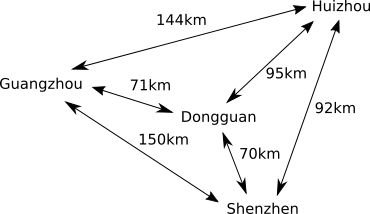
\includegraphics[scale=0.5]{images/traveller.png} 
     	\vspace*{-0.5em}
		%\caption{What is the route with the shortest distance to visit all the cities?}
	\end{figure}	
	
	A naïve approach would be: computing all the possible routes and keep the one with the shortest total distance.
	
	\pause
	
	\begin{alertblock}{This approach is not suited when there are too many cities}
	\begin{itemize}
	\item {For 4 cities: 24 distance additions (few miliseconds)}
	\item {For 20 cities: $2\times 10^{18}$ distance additions (more than 1 million years...)}
	\end{itemize}
	\end{alertblock}
	
	\end{frame}	
	
	\subsection{Evaluating the complexity}
	
	\begin{frame}	
	
	\begin{block}{How can I know if my algorithm design is appropriate enough?}
	As mentioned before, by evaluating the complexity!
	\end{block}
	
	\pause
	
	\begin{exampleblock}{Complexity}
	It gives the \textbf{number of fundamental operations} that will be processed by the algorithm according to the \textbf{amount of input data}. Example: the number of distance additions (see previous slide).
	\end{exampleblock}
	
	\pause
	
	Knowing the complexity permits to...
		
	\begin{itemize}
	\item {... indirectly estimate the total time of execution}
	\item {... indirectly estimate the total memory consumption\footnote{Note that most of the time when people refer to \textit{complexity} they mean time related complexity (known as \textit{time complexity})}}
	\end{itemize}		
		
	%Indeed, a fundamental operation is related to a finite amount of time consumption (depending on the machine) and a finite amount of memory consumption.		
		
	\end{frame}
	
	%\subsection{Notion of fundamental operation}
	
	\begin{frame}
	
	\begin{exampleblock}{Fundamental operation}
	Fundamental operations are the building-blocks of the algorithm\footnotemark
	\end{exampleblock}	
	A fundamental operation ...	
	\begin{itemize}
	
	\item {... has a \textbf{well defined time and memory consumption}
		\begin{itemize}
			\item {Ex: value assignation of an addition, computing a surface, etc.}
		\end{itemize}				
	}
	\item {... \textbf{can be complex}
	\begin{itemize}
	\item{i.e: "absorbing" a bunch of smaller and various operations}
	\item{Ex: algebra operations on an input vector (machine learning)}
	\end{itemize}
	}
		
	\end{itemize}		

	\pause
	
	\begin{alertblock}{What to do if there are several fundamental operations?}
	In case there are several fundamental operations (no further "absorption" or simplification is possible to have one unique fundamental operation): the final complexity will be the addition of all the complexities.\end{alertblock}
	
	\footnotetext{Note that: two algorithms can only be compared if they have the same fundamental operations.}
	
	\end{frame}
		
	\subsection{Example of complexity calculus}	
	
	\begin{frame}
	
	\begin{exampleblock}{Recall}
	The complexity is the \textbf{number of fundamental operations} that will be processed by the algorithm according to the \textbf{amount of input data}.
	\end{exampleblock}
	
	Example: looking for the value $x$ in the array of integer $T$ (of size $N$)
	
	\begin{center}    
    \scalebox{0.75} {
    %\begin{minipage}
    \begin{algorithm}[H]
 	\KwData{$T$(sorted by increasing values)}
 	%\KwResult{how to write algorithm with \LaTeX2e }
	$k=0$\; 	
 	\While{$k < N$}{
 		\eIf{$T[k] >= x$}{
 			return $k$\;
 		}
 		{ $k=k+1$\;}
 	}
 	\caption{pseudo-code of basic search algorithm}
	\end{algorithm}	
	%\end{minipage}
	}
	\end{center} 
	
	\begin{itemize}
	\item{Here the fundamental operation is the conditional test "if"}
	\item{Complexity: at best 1, at worst $N$ and in average: $\frac{N}{2}$ operations}
	\end{itemize}	
			
	\end{frame}
	
	\subsection{Complexity definitions}
	
	\begin{frame}		
	
	\begin{exampleblock}{Three complexity definitions}
	There are three complexity definitions: \textbf{complexity at best},  \textbf{complexity at worst} and \textbf{complexity in average}. The complexity at worst and in average are the most used (because there are pessimistic predictions).	
	\end{exampleblock}	
	
	\begin{itemize}
	\item {complexity at best = minimum number of required operations}
	\item {complexity at worst = maximum number of operations we could have}
	\item {complexity in average = most likely number of operations}	
	\end{itemize}	
	
	\vspace*{1em}	
	
	complexity at best $<$ complexity in average $<$ complexity at worst
	
	\end{frame}
	
	\begin{frame}
	
	Example 2: looking for the value $x$ in the array of integer $T$	 (of size $N$) with a dichotomic search
	
	\begin{center}    
    \scalebox{0.75} {
    %\begin{minipage}
    \begin{algorithm}[H]
 	\KwData{$T$(sorted by increasing values)}
 	%\KwResult{how to write algorithm with \LaTeX2e }
	$k=0$; $i=0$; $j=N$\;
 	\While{$i < j$}{
 		$k=(i+j)/2$\;
 		\eIf{$T[k] < x$}{
 			$i=k+1$\;
 		}{
 			$j=k$\;
 		}
 	}
 	\If{$i == N-2$ and $T[i] < x$}{ $i=N-1$\; }
 	return $i$\;
 	\caption{pseudo-code of dichotomic search algorithm}
	\end{algorithm}	
	%\end{minipage}
	}
	\end{center} 
	
	Here, the complexity at worst = $log_2N$	(much better than the basic search!)
	
	\end{frame}	
	
	\begin{frame}
	
	Indeed:
	
	\begin{enumerate}
		\item {At each loop, N is divided by 2 and the smallest instance size is 1, so we have: $1 \leq \frac{N}{2^{number\ operations}}$}
		\item {By multiplying by $2^{number\ operations}$ we get: $2^{number\ operations} \leq N$}
		\item {By composing with $log$ we get: $number\ operations \times log(2) \leq log(N)$}
		\item {Finally we get: $number\ operations \leq log_2(N)$}	
	\end{enumerate}	 	
	
	\end{frame}	
		
	\subsection{The big O notation}	
	
	\begin{frame}	
	
	\begin{exampleblock}{The big $O$ notation}
	The complexity is most of the time expressed with the big $O$ notation	:
	\begin{itemize}
	\item{$f = O(g) \Leftrightarrow $ f is \textit{dominated} by g}
	\item{$f = O(g) \Leftrightarrow \exists n_o $ such that for all $n > n_o, f(n) \leq c \times g(n)$ }
	\end{itemize}
	\end{exampleblock}	
	
	The big $O$ notation is well suited for complexity analysis because it represents well the \textbf{order of magnitude} and the \textbf{evolution with respect to the size}.
				
	\begin{figure}
		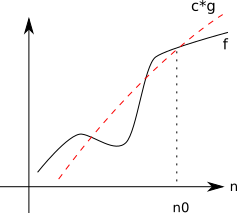
\includegraphics[scale=0.6]{images/o_notation_example.png} 
     	\vspace*{-0.6em}
		\caption{$f$ is dominated by $g$}
		\end{figure}	
			
	\end{frame}	
	
	\begin{frame}
		
	big $O$ notations of complexities:
	
	\begin{itemize}
	\item {$N \Rightarrow O(N)$} 
	\item {$log_2(N) \Rightarrow O(log_2(N) \Rightarrow O(log(N))$}	
	\item {$2\times N^2 \Rightarrow O(N^2)$}
	\item {$5\times N^3 + 200 \times N^2 + 15 \Rightarrow O(N^3)$}
	\item {$2\times log_2(N) + 15\times ln(N) \Rightarrow O(log(N))$}
	\item {$2^{64} \Rightarrow O(1)$}
	\item {$log(N^{10}) + 2\sqrt{N} \Rightarrow O(\sqrt{N})$}	
	\item {$2^N + N^{1000} \Rightarrow O(2^N)$}
	\item {...}
	\end{itemize}		
	
	%\begin{block}{Recall}
	%$f = O(g) \Leftrightarrow \exists n_o $ such that for all $n > n_o, f(n) \leq c \times g(n)$
	%\end{block}
	
	\end{frame}	
	
	\subsection{Tips to find the complexity}	
	
	\begin{frame}
	
	Let's assume $f$  is our functional operation, then:
	
	\begin{columns}[c]
	\column{.5\textwidth}
	\begin{center}  
    \scalebox{0.55} {
    %\begin{minipage}
    \begin{algorithm}[H]
	 \For{$i\gets0$ \KwTo $N$}{
    	$f()$
    }
	\end{algorithm}	
	}
	\end{center} 
	\column{.5\textwidth}
	$\Longrightarrow O(N)$
	\end{columns}	
	
	\begin{columns}[c]
	\column{.5\textwidth}
	\begin{center}    
    \scalebox{0.55} {
    %\begin{minipage}
    \begin{algorithm}[H]
	 \For{$i\gets0$ \KwTo $N$}{
	 	\For{$j\gets0$ \KwTo $N$}{
    		$f()$
    		}
    }
	\end{algorithm}	
	}
	\end{center} 
	\column{.5\textwidth}
	$\Longrightarrow O(N^2)$
	\end{columns}	
	
	\begin{columns}[c]
	\column{.5\textwidth}
	\begin{center}    
    \scalebox{0.55} {
    %\begin{minipage}
    \begin{algorithm}[H]
	 \For{$i\gets0$ \KwTo $N$}{
	 	\For{$j\gets0$ \KwTo $N$}{
	 		\For{$j\gets0$ \KwTo $N$}{
    		$f()$
    		}
    	}
    }
	\end{algorithm}	
	}
	\end{center}
	\column{.5\textwidth}
	$\Longrightarrow O(N^3)$
	\end{columns}
		
	\begin{columns}[c]
	\column{.5\textwidth}
	\begin{center}    
    \scalebox{0.55} {
    %\begin{minipage}
    \begin{algorithm}[H]
	 \For{$i\gets0$ \KwTo $N$}{
	 	\For{$j\gets0$ \KwTo $M$}{
	 		\For{$j\gets0$ \KwTo $P$}{
    		$f()$
    		}
    	}
    }
	\end{algorithm}	
	}
	\end{center}
	\column{.5\textwidth}
	$\Longrightarrow O(N\times M\times P)$	
	\end{columns}
		
	\end{frame}		
	
	\begin{frame}
	
	Complexity examples of well-known algorithms:	
	
	\begin{itemize}
	
	\item{\textbf{$O(1)$}: accessing array index, inserting a node in linked list, pushing and popping (stack), insertion and removal from queue, etc.}

	\item{\textbf{$O(n)$}: traversing an array, traversing a linked list, linear search, delete element in a not sorted linked list, comparing two strings}

	\item{\textbf{$O(log(N))$}: dichotomy or binary search, finding largest/smallest number in a binary search tree,  calculating Fibonacci Numbers, etc.}

	\item{\textbf{$O(N\times log(N))$}: merge sort, heap sort, quick sort, etc.}

	\item{\textbf{$O(N^2)$}: bubble sort, insertion sort, selection sort, traversing a simple 2D array, etc.	}
	
	\end{itemize}
	
	
	\end{frame}
	
	\subsection{Examples of time and memory consumption estimations}	
	
	\begin{frame}	
	
	\begin{tabular}{ c | c | c | c | c | c | c | c }
	Size & 1 & $log(N)$ & N & $N \times log(N)$ & $N^2$ & $N^3$ & $2^N$ \\ 
	& & \tiny{(logarithmic)} & \tiny{(linear)} & \tiny{(N-logarithmic)} & \tiny({quadratic)} & \tiny{(cubic)}  & \tiny{(exponential)} \\ \hline
	$10^2$ & 1$\mu$s & 7$\mu$s & 0.1ms & 0.7ms & 10ms & 1s & $4\times 10^7$Gy \\
	$10^3$ & 1$\mu$s & 10$\mu$s & 1ms & 10ms & 1ms & 17min & X \\
	$10^4$ & 1$\mu$s & 13$\mu$s & 10ms & 130ms & 1.7ms & 12d & X \\		
	$10^5$ & 1$\mu$s & 17$\mu$s & 0.1s & 1.7s & 2.8h & 32y & X \\		
	$10^6$ & 1$\mu$s & 20$\mu$s & 1s & 20s & 12d & 32Ky & X \\	
	\end{tabular}	
	
	\end{frame}
	
	\begin{frame}
	
		\begin{tabular}{ c | c | c | c | c | c | c | c }
	Time & 1 & $log(N)$ & N & $N \times log(N)$ & $N^2$ & $N^3$ & $2^N$ \\ 
	& & \tiny{(logarithmic)} & \tiny{(linear)} & \tiny{(N-logarithmic)} & \tiny{(quadratic)} & \tiny{(cubic)}  & \tiny{(exponential)} \\ \hline
	1s & X & X & 1M & 63K & 1K & 100 & 20 \\
	1min & X & X & 60M & 3M & 7K & 400 & 26 \\
	1h & X & X & 3.6G & 130M & 60K & 1.5K & 32 \\		
	1d & X & X & 96G & 3G & 300K & 4.4K & 36 \\		
	\end{tabular}	
	
	\vspace*{0.5em}
	
	\begin{itemize}
	\item {1 day with linear time complexity: 
		\begin{itemize}
			\item {$96\times 10^9$ fundamental operations are done}
			\item {If 1 fundamental operation generates 1Byte, then total storage = 96GO}			
		\end{itemize}				
	}
	\item {1 second with quadratic time complexity: 
		\begin{itemize}
			\item {$1\times 10^3$ fundamental operations are done}
			\item {If 1 fundamental operation generates 1MO, then total storage = 1GO}	
		\end{itemize}			
	}	
	\end{itemize}
	
	\pause	
	
	\begin{block}{Time complexity, space complexity, what's the difference?}
	Time complexity focuses on the \textbf{fundamental operation iterations}, space complexity on the \textbf{space consumption}.
	\end{block}		
		
	\end{frame}
	
	\section{Conclusion}	
	
	\begin{frame}
		
	When designing your algorithm ...
	\begin{itemize}
	\item {...optimize well your \textbf{memory usage} if you need/can:
		\begin{itemize}
			\item {main memory is fast but small}
			\item {mass memory is slow but big}
			\item {limiting the number of mass memory accesses is good for performance}
			\item {big intermediary results should be saved on mass memory for space}
				
		\end{itemize}			
	}
	
	\item {...optimize your \textbf{time complexity}:
		\begin{itemize}
			\item {a time complexity $< N^2$: we can process almost all input size}
			\item {a time complexity between $N^2$ and $N^3$: intermediate input size}
			\item {a time complexity $> N^3$: small input size}		
		\end{itemize}		
	}
	\item {...don't forget to have a look to your \textbf{space complexity}:
		\begin{itemize}
			\item {it may not finish because the memory got completely saturated!}
		\end{itemize}
	}			
	\end{itemize}	
	
	\begin{alertblock}{Note}
	A more powerful computer does not "improve the complexity". It only \textit{reduces} the time spent on each fundamental operation. But the issue is the same.
	\end{alertblock}

	
	\end{frame}

	




\end{document}